\section{Principali tipologie di densità}

\begin{defn}
    \textbf{Densità uniforme su [a, b]} \\
    Sia data $ X $ con densità $ f(x) $
    \begin{equation*}
        f(x; a, b) = \begin{cases}
            \frac{1}{b-a} & a \leq x \leq b \\
            0   &    \text{altrimenti}
        \end{cases}
    \end{equation*}

    Il \textbf{valore atteso è} $ \dfrac{a + b}{2} $. La \textbf{varianza} è $
    \dfrac{(b - a)^2}{12}$

    \begin{figure}[htbp]
        \centering

        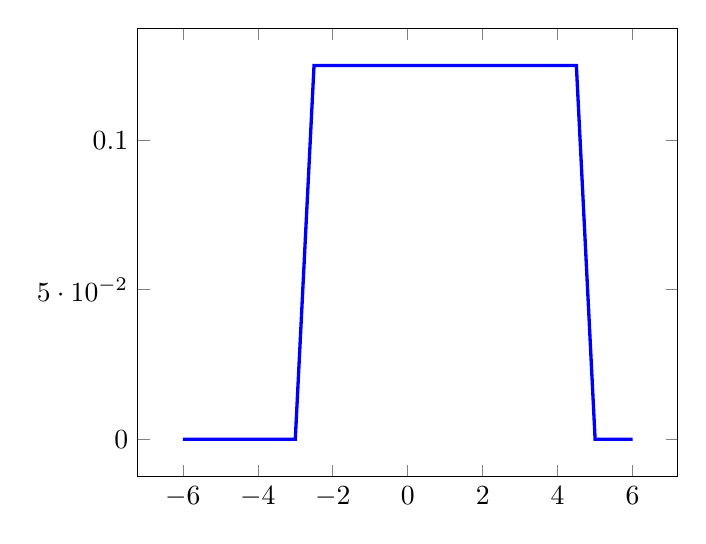
\begin{tikzpicture}[declare function={unipdf(\x,\xl,\xu)=
        (\x>\xl)*(\x<\xu)*1/(\xu-\xl);}]
            \begin{axis}[] \addplot[very thick, blue][domain=-6:6]
                {unipdf(x,-3,5)};
            \end{axis}
        \end{tikzpicture}
        \caption{Densità di probabilità uniforme di parametri $a = -3$ e $b = 5$}
        \label{uniform}
    \end{figure}


    La funzione di ripartizione $F$ è definita come
    \begin{equation*}
        F(x) = \int_{-\infty}^x f(t) dt = \begin{cases}
            0 & x \leq a \\
            \frac{x-a}{b-a} & a < x < b \\
            1 & x \geq b
        \end{cases}
    \end{equation*}
    $ F $ è la funzione di ripartizione in tutti i punti in cui $ f $ è continua
    \begin{equation*}
        f(x) = \frac{dF(x)}{dx}
    \end{equation*}

    \begin{figure}[htbp]
        \centering

        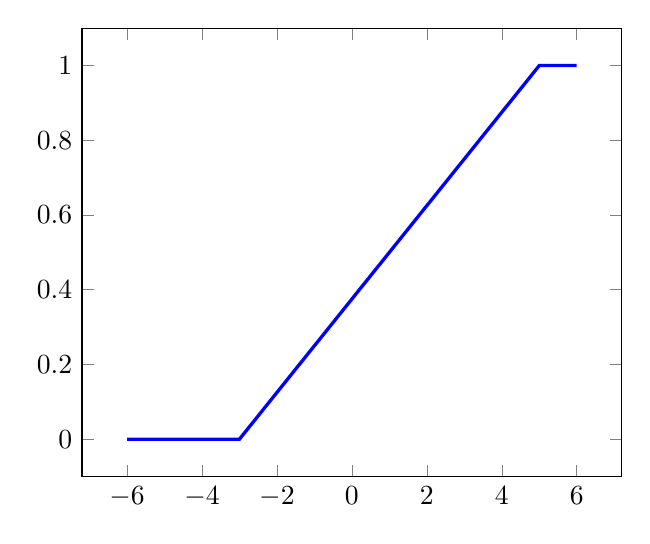
\begin{tikzpicture}[declare function={func(\x,\a,\b) = and(\x > \a, \x <
            \b) * ((\x - \a)/(\b - \a)) + (\x >= \b);}]
            \begin{axis}[] \addplot[very thick, blue][domain=-6:6]
                {func(x,-3,5)};
            \end{axis}
        \end{tikzpicture}
        \caption{Funzione di ripartizione della densità di probabilità uniforme di parametri $a = -3$ e $b = 5$}
        \label{uniformpart}
    \end{figure}

\end{defn}

\begin{defn}
    \textbf{Densità esponenziale di parametro} $ \lambda > 0 $ \\
    Sia data la densità
    \begin{equation*}
        f(x) = \begin{cases}
            \lambda e^{-\lambda x} & x \geq 0 \\
            0 & x < 0
        \end{cases}
    \end{equation*}

    Il valore atteso è $ \dfrac{1}{\lambda} $. La speranza è
    $\dfrac{1}{\lambda^2}$

    \begin{figure}[htbp!]
        \centering

        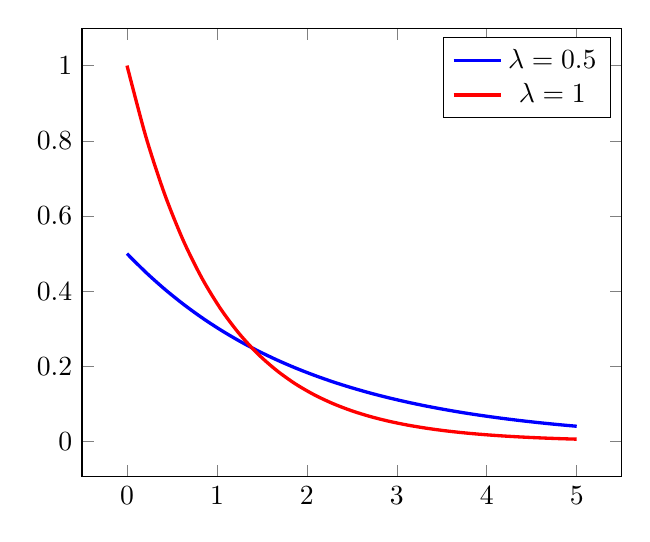
\begin{tikzpicture}[declare function={func(\x,\lambda) =
            (\lambda*e^(-\lambda*\x));}]
            \begin{axis}[smooth,
                legend entries={$\lambda=0.5$,$\lambda=1$}
                ] \addplot[very thick, blue][domain=0:5]
                {func(x,0.5)}; \addplot[very thick, red][domain=0:5]
                {func(x,1)};
            \end{axis}
        \end{tikzpicture}
        \caption{Densità di probabilità esponenziale}
        \label{exparam}
    \end{figure}

    \begin{figure}[htbp!]
        \centering

        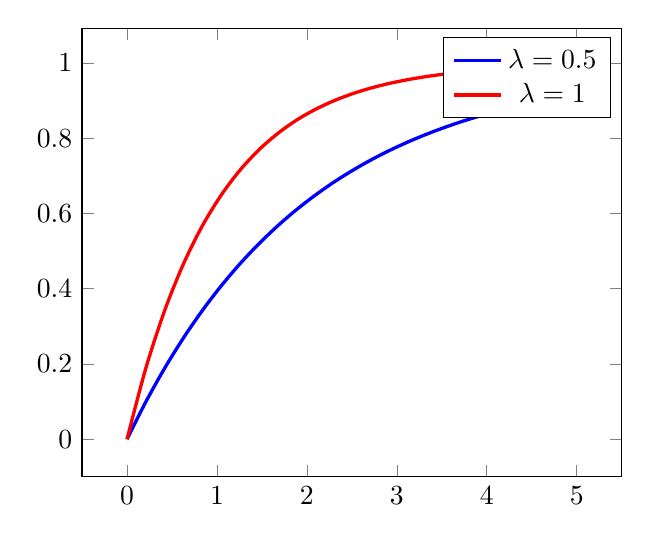
\begin{tikzpicture}[declare function={func(\x,\lambda) = (1 -
            e^(-\lambda*\x));}]
            \begin{axis}[smooth,
                legend entries={$\lambda=0.5$,$\lambda=1$}
                ] \addplot[very thick, blue][domain=0:5]
                {func(x,0.5)}; \addplot[very thick, red][domain=0:5]
                {func(x,1)};
            \end{axis}
        \end{tikzpicture}
        \caption{$P(X \leq x)$ (funzione di ripartizione) di un'esponenziale di parametro $\lambda = 0.5$ (blu) e $\lambda = 1$ (rosso)}
        \label{exparam2}
    \end{figure}

    La funzione di ripartizione $ F $ è
    \begin{equation*}
        F(x) = \int_{-\infty}^{x} f(t) dt = \begin{cases}
            0 & x \leq 0 \\
            1 - e^{-\lambda x} & x > 0 \\
        \end{cases}
    \end{equation*}

\end{defn}

% //TODO ???????
\begin{note}
    Se X ha densità

    \begin{equation*}
        \p{X = x} = \int_x f(t) dt = 0
    \end{equation*}
\end{note}

\begin{defn}
    \textbf{Densità di Cauchy} \\
    La densità di Cauchy (detta anche distribuzione di Cauchy o distribuzione di
    Lorentz) è una particolare funzione di densità che descrive nel piano
    euclideo l'intersezione tra l'asse delle ascisse ed una retta passante per
    un punto fissato ed inclinata ad un angolo che segue la distribuzione
    continua uniforme. I momenti di una distribuzione di Cauchy non sono
    definiti.

    \begin{equation*}
        \begin{aligned}
            f(x) = \frac{1}{\pi (1+x)^2}
        \end{aligned}
    \end{equation*}


    \begin{figure}[htbp!]
        \centering

        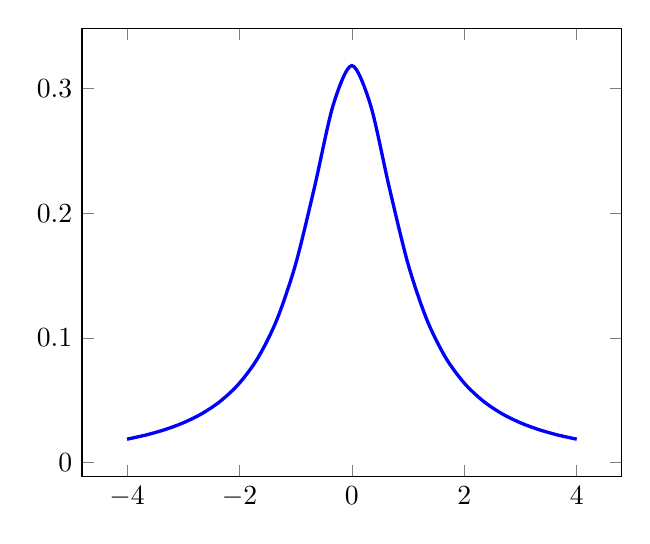
\begin{tikzpicture}[declare function={func(\x) = (1/(pi * (1 +
            \x^2)));}]
            \begin{axis}[smooth] \addplot[very thick, blue][domain=-4:4]
                {func(x)};
            \end{axis}
        \end{tikzpicture}
        \caption{Densità di probabilità di Cauchy}
        \label{cauchy}
    \end{figure}


    \begin{prop}
        La distribuzione di Cauchy è una densità di probabilità.
    \end{prop}

    \begin{proof}
        \begin{equation*}
            \begin{aligned}
                \frac{1}{\pi} \int_{-\infty}^{+\infty} \frac{1}{1 + x^2} dx = \frac{1}{\pi} \lim_{M \to +\infty} \int_{-M}^{M} \frac{dx}{1 + x^2} \\
                = \frac{1}{\pi} \lim_{M \to +\infty} \left( \arctan(M) - \arctan(-M) \right) = \frac{1}{\pi} \left( \frac{\pi}{2} + \frac{\pi}{2} \right) = 1
            \end{aligned}
        \end{equation*}
    \end{proof}

    \begin{prop}
        La densità di Cauchy non ha momenti.
    \end{prop}

    \begin{proof}
        \begin{equation*}
            \begin{aligned}
                \frac{1}{\pi} \int_{-\infty}^{+\infty} \frac{\abs{x}{}}{1 + x^2} dx = \frac{1}{\pi} \int_{0}^{+\infty} \frac{2x}{1 + x^2} dx =
                \frac{1}{\pi} \left[ \log(1 + x^2) \right]_{0}^{+\infty} = - \frac{1}{\pi} \cdot 0 + \frac{1}{\pi} \cdot +\infty = +\infty \\
                \implies \nexists \E{X}
            \end{aligned}
        \end{equation*}
    \end{proof}
\end{defn}

\begin{defn}
    \textbf{Funzione Gamma $\Gamma$} \\
    La funzione $\Gamma$ è un'estensione della funzione fattoriale ai numeri
    complessi. È definita su tutti i numeri complessi con parte reale $> 0$.
    Per definire la \textbf{densità di probabilità $\Gamma$}, utilizzeremo la
    funzione $@G$ definita solo per i numeri reali positivi.

    \begin{equation*}
        \begin{aligned}
            r > 0 \implies \Gamma(r) = \int_{0}^{+\infty} x^{r - 1}e^{-x} dx
        \end{aligned}
    \end{equation*}

    \begin{prop}
        Sui reali positivi, la funzione $\Gamma(r+1) = r\Gamma(r)$. Sui numeri
        naturali, allora $\Gamma(n+1) = n!$.
    \end{prop}

    \begin{proof}
        \begin{equation*}
            \begin{aligned}
                \Gamma(r+1) = \int_{0}^{+\infty} x^r e^{-x} dx = \left[ -x^r e^{-x} \right]_{0}^{+\infty} + \int_{0}^{+\infty} rx^{r-1} e^{-x} dx \\
                = \lim_{x \to +\infty} (-x^r e^{-x}) - (0e^0) + r \int_{0}^{+\infty} x^{r-1} e^{-x} dx \\
                \text{osservando che $\lim_{x \to +\infty} (-x^r e^{-x})$ tende a 0} \\
                \Gamma(r+1) = r \int_{0}^{+\infty} x^{r-1} e^{-x} dx = r \Gamma(r)
            \end{aligned}
        \end{equation*}
    \end{proof}
    
    Completiamo la definizione della funzione $\Gamma$:

    \begin{equation*}
        \begin{aligned}
            n \in \N \implies \Gamma(n) = \begin{cases}
                \Gamma(n) = \Gamma(1) = 1 & n = 1 \\
                \Gamma(n) = (n-1)! & n > 1
            \end{cases}
        \end{aligned}
    \end{equation*}
\end{defn}

\begin{defn}
    \textbf{Distribuzione $\Gamma$} \\
    Dopo aver definito la funzione $\Gamma$, possiamo definire la densità di
    probabilità per la distribuzione $\Gamma$. I due parametri della densità
    vengono detti forma ($r$) e scala ($\lambda$) della distribuzione.

    \begin{equation*}
        \begin{aligned}
            \Gamma(r, \lambda) = f(x) = \begin{cases}
                \left( \dfrac{1}{\Gamma(r)} \right) \lambda^r  x^{r-1} e^{-\lambda x} & x \geq 0 \\
                0 & x < 0
            \end{cases}
        \end{aligned}
    \end{equation*}

    Il \textbf{valore atteso} è $\dfrac{r}{\lambda}$, la \textbf{varianza} è $\dfrac{r}{\lambda^2}$.

    Si nota come una densità esponenziale di parametro $\lambda$ sia uguale ad
    una densità $\Gamma$ di parametri $r = 1, \lambda = \lambda$. Infatti, le
    densità esponenziali e le densità $\chi^2$ sono casi speciali della
    distribuzione $\Gamma$

    \begin{figure}[htbp!]
        \centering

        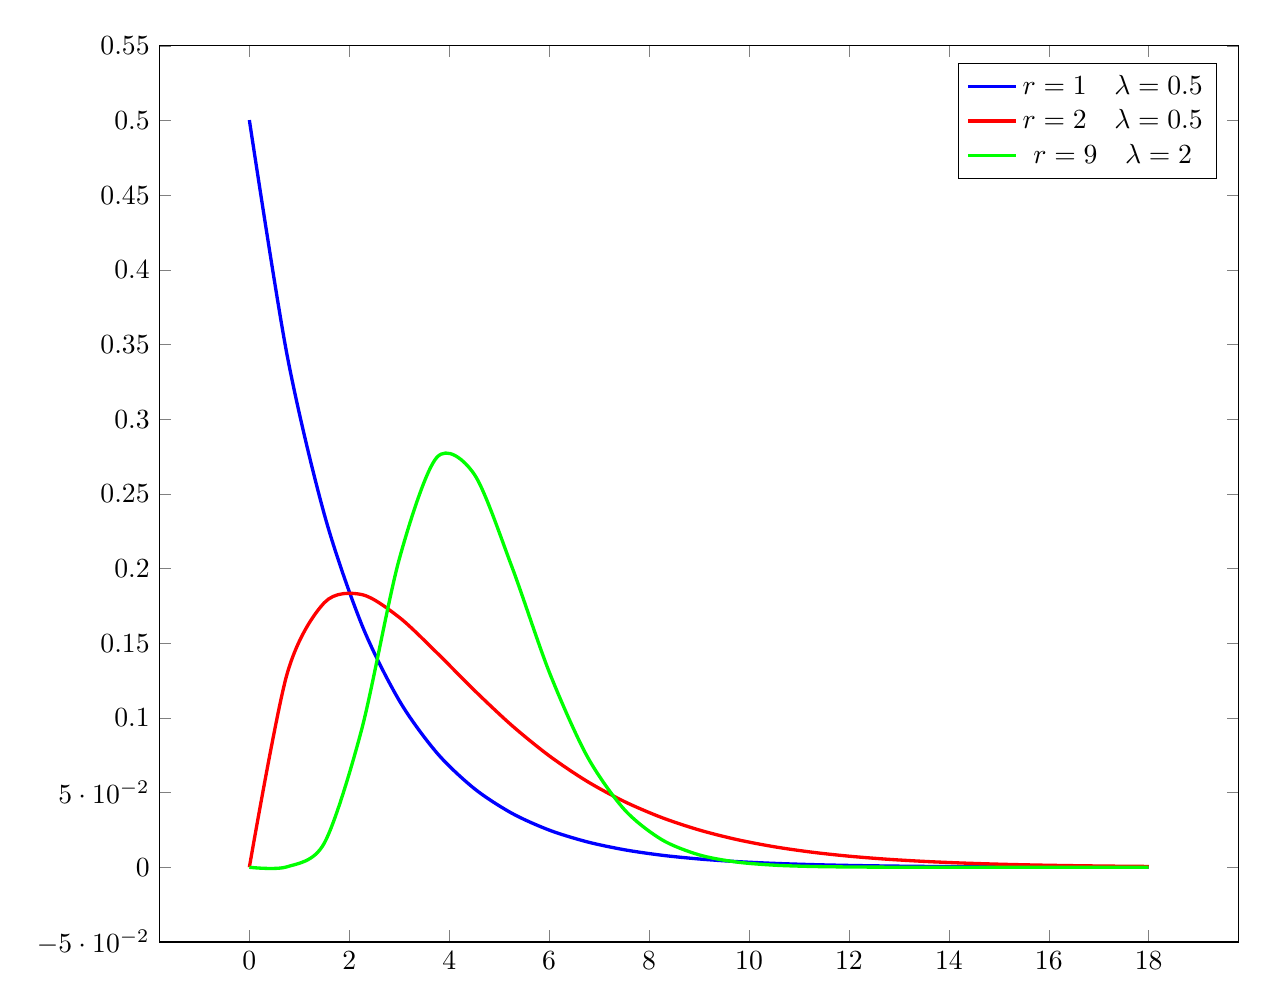
\begin{tikzpicture}[
            declare function={gamma(\z)=
            (2.506628274631*sqrt(1/\z) + 0.20888568*(1/\z)^(1.5) + 0.00870357*(1/\z)^(2.5) - (174.2106599*(1/\z)^(3.5))/25920 - (715.6423511*(1/\z)^(4.5))/1244160)*exp((-ln(1/\z)-1)*\z);},
            declare function={gammapdf(\x,\k,\theta) = \x^(\k-1)*exp(-\x/\theta) / (\theta^\k*gamma(\k));}
        ]
            \begin{axis}[scale=2, smooth,
                legend entries={$r=1\quad \lambda=0.5$,$r=2\quad \lambda=0.5$, $r=9\quad \lambda=2$}
                ]
                \addplot[very thick, blue][domain=0:18]{gammapdf(x, 1, 2)};
                \addplot[very thick, red][domain=0:18]{gammapdf(x, 2, 2)};
                \addplot[very thick, green][domain=0:18]{gammapdf(x, 9, 0.5)};
            \end{axis}
        \end{tikzpicture}
        \caption{Densità di probabilità $\Gamma$}
        \label{gammapdf}
    \end{figure}

    \begin{prop}
        La densità $\Gamma(r, \lambda)$ è una densità di probabilità
    \end{prop}

    \begin{proof}
        Il prodotto di numeri positivi è positivo, quindi la funzione di densità
        $f \geq 0$. Rimane da dimostrare che $\int_{-\infty}^{+\infty} f(x) dx =
        1$ per dimostrare che la funzione data da $\Gamma(r, \lambda)$ è una
        di probabilità. Conosciamo intanto $\int_{-\infty}^{0} f(x) dx = 0$.

        \begin{equation*}
            \begin{aligned}
                \int_{0}^{+\infty} \lambda^r x^{r-1} e^{-\lambda x} dx = \int_{0}^{+\infty} (\lambda x)^{r-1} e^{-\lambda -1} dx = \\
                \text{Risolvendo per sostituzione: } t = \lambda x \implies dt = \lambda dx \\
                = \int_{0}^{+\infty} t^{r-1} e^{-t} dt = \Gamma(r) \\
                \implies \int_{-\infty}^{+\infty} f(x) dx = \dfrac{1}{\Gamma(r)} \Gamma(r) = 1
            \end{aligned}
        \end{equation*}
    \end{proof}
\end{defn}

\begin{defn}
    \textbf{Formula dei momenti della distribuzione $\Gamma$} \\
    Definiamo una formula per calcolare il momento $n$-esimo di una variabile
    aleatoria con densità data dalla distribuzione $\Gamma$.

    \begin{equation*}
        \begin{aligned}
        X \sim \Gamma(r, \lambda) \implies \\
        \E{X} = \frac{\Gamma(r + 1)}{\Gamma(r) \lambda} = \frac{\Gamma(r) (r)}{\Gamma(r) \lambda} = \frac{r}{\lambda} \\
        \E{X^2} = \frac{\Gamma(r + 2)}{\Gamma(r) \lambda^2} = \frac{r(r+1)}{\lambda^2}
        \end{aligned}
    \end{equation*}

    Ed in generale:

    \begin{equation*}
        \begin{aligned}
           X \sim \Gamma(r) \land n \in \N \implies \E{X^n} = \frac{\Gamma(r + n)}{\Gamma(r) \lambda^n}
        \end{aligned}
    \end{equation*}

    \begin{proof}
        \begin{eqnarray*}
            \E{X^n} &=& \frac{1}{\Gamma(r)} \int_{0}^{+\infty} x^n \lambda^r x^{r-1} e^{-\lambda x} dx  \\
            &=& \frac{1}{\Gamma(r)} \cdot \frac{1}{\lambda^n} \int_{0}^{+\infty} \lambda^{r+n} x^{n + r -1} e^{-\lambda x} dx \\
            &=& \frac{\Gamma(r + n)}{\Gamma(r) \lambda^n}
        \end{eqnarray*}
    \end{proof}

\end{defn}

\begin{defn}
    \textbf{Somma di variabili aleatorie indipendenti con distribuzione $\Gamma$} \\

    \begin{equation*}
        \begin{aligned}
            X \sim \Gamma(r_X, \lambda) \land Y \sim \Gamma(r_Y, \lambda) \land X,Y \text{  indipendenti} \\
            \implies (X + Y) \sim \Gamma(r_X + r_Y, \lambda)
        \end{aligned}
    \end{equation*}

\end{defn}


\begin{defn}
    \textbf{Distribuzione normale (Gaussiana)} \\
    La distribuzione Gaussiana ha una funzione di densità a forma di campana. È
    utilizzata per rappresentare variabili aleatorie a valori reali che sono
    prodotte dalla somma di tanti piccoli risultati. Ad esempio, la
    distribuzione normale viene utilizzata per modellare l'altezza della
    popolazione, perché l'altezza può essere il risultato di tanti piccoli
    fattori genetici e ambientali.

    Sia data la densità $f(x;\mu, \sigma^2)$ dove $\mu$ è il parametro che
    rappresenta il valore atteso e $\sigma^2$ rappresenta la varianza. Si indica
    comunemente con $N(\mu, \sigma^2)$. Dal grafico si nota che la campana si sposta orizzontalmente al
    variare di $\mu$, mentre al variare della varianza $\sigma^2$ la campana
    "cambia forma".

    \begin{equation*}
        \begin{aligned}
            N(\mu, \sigma^2) = f(x) = \frac{1}{\sigma \sqrt{2\pi}} e^{-\dfrac{(x - \mu)^2}{2 \sigma^2}}
        \end{aligned}
    \end{equation*}

    \pgfmathdeclarefunction{gauss}{2}{%
     \pgfmathparse{1/(#2*sqrt(2*pi))*exp(-((x-#1)^2)/(2*#2^2))}%
    }

    \begin{figure}[htbp!]
        \centering

        \begin{tikzpicture}[]
            \begin{axis}[scale=2.3, smooth,
                legend entries={$\mu=0\quad \sigma^2=1.44$, $\mu=0.66\quad \sigma^2=0.22$, $k=1.44\quad \sigma^2=3.68$}
                ]
                \addplot[very thick, blue][domain=-5:6]{gauss(0, 1.2)};
                \addplot[very thick, red][domain=-5:6]{gauss(0.66, 0.47)};
                \addplot[very thick, green][domain=-5:6]{gauss(1.44, 1.92)};
            \end{axis}
        \end{tikzpicture}
        \caption{Densità di probabilità Gaussiana}
        \label{gaussian}
    \end{figure}
\end{defn}

\FloatBarrier

\begin{defn}
    \textbf{Densità Gaussiana Standard} \\
    La densità Gaussiana $N(0,1)$ di
    parametri $\mu = 0$ e $\sigma^2 = 1$ viene detta \textbf{densità Gaussiana
    standard}. Si usa comunemente la lettera greca $\phi$ (phi) per indicare la
    funzione di densità e la controparte maiuscola $\Phi$ per indicare la funzione di ripartizione (CDF).

    \begin{equation*}
        \begin{aligned}
            \phi(x) = \frac{1}{\sqrt{2 \pi}} e^{-\dfrac{x^2}{2}}
        \end{aligned}
    \end{equation*}

    La funzione di ripartizione è:

    \begin{equation*}
        \begin{aligned}
            \Phi(x) = \frac{1}{\sqrt{2 \pi}} \int_{-\infty}^{x} e^{-(t^2/2)} dt
        \end{aligned}
    \end{equation*}

    \begin{prop}
        Una variabile $X \sim N(0,1)$ con densità Gaussiana standard ha tutti i
        momenti.
    \end{prop}

    \begin{proof}
        \begin{equation*}
            \begin{aligned}
                \frac{1}{\sqrt{2 \pi}} \int_{-\infty}^{+\infty} \abs{x}^n e^{-(x^2/2)} dx < +\infty
            \end{aligned}
        \end{equation*}
        Sapendo che $e^{-(x^2/2)}$ tende a 0 per $x = +\infty$ e per $x = -\infty$
    \end{proof}
\end{defn}

\begin{defn}
    \label{engauss}
    \textbf{Momenti $n$-esimi di una Gaussiana standard} \\
    Per calcolare il \textbf{momento $n$-esimo} di una gaussiana standard
    definiamo una funzione Mo($n$) come

    \begin{itemize}
        \item Se $n$ è dispari:
        \begin{equation*}
            \begin{aligned}
                n = 2h + 1 \implies \text{Mo}(n) = \E{X^{2h+1}} = \frac{1}{\sqrt{2 \pi}}
                \int_{-\infty}^{+\infty} x^{2h+1} e^{-(x^2/2)} dx = 0
            \end{aligned}
        \end{equation*}
        \item Se $n$ è pari:
        \begin{equation*}
            \begin{aligned}
                n = 2h \implies \text{Mo}(n) = \E{X^{2h}} = (2h-1) \E{X^{2h-2}} = (n-1) \text{Mo}(n-2)
            \end{aligned}
        \end{equation*}
    \end{itemize}

    Ad esempio, $\E{X^2} = 1$ e $\E{X^4} = 3 \cdot \E{X^2} = 3$ .
\end{defn}

\begin{defn}
    \textbf{Varianza di una Gaussiana standard} \\
    Dalla definizione \ref{engauss} si ottiene che la varianza di una variabile
    aleatoria $X \sim N(0,1)$ è
    \begin{equation*}
        \begin{aligned}
            \var{X} = \E{X^2} - \E{X}^2 = 1 - 0^2 = 1
        \end{aligned}
    \end{equation*}
\end{defn}

\begin{defn}
    \textbf{Conversione di una variabile aleatoria da Gaussiana qualsiasi a Gaussiana standard} \\
    \begin{prop}
        Si può sempre pensare una variabile aleatoria $X \sim N(\mu, \sigma^2)$
        nella forma $\sigma X + m$ con $X \sim N(0, 1)$.
    \end{prop}

    \begin{proof}
        Siano dati:
        \begin{equation*}
            \begin{aligned}
                \mu \in \R, \quad \sigma > 0, \quad X \sim (N(0,1) = f(x)), \quad Y = \sigma X + \mu, \quad Y \sim g(y)\\
                y = \sigma x + \mu \implies x = \dfrac{y-\mu}{\sigma}\\
                \implies g(y) = \frac{1}{\sigma \sqrt{2 \pi}} e^{- \dfrac{1}{2} \left( \dfrac{y - m}{\sigma}\right)^2 }\\
                \implies Y \sim N(\mu, \sigma^2) \implies \E{Y} = \mu \land \var{Y} = \sigma^2
            \end{aligned}
        \end{equation*}
    \end{proof}

\end{defn}

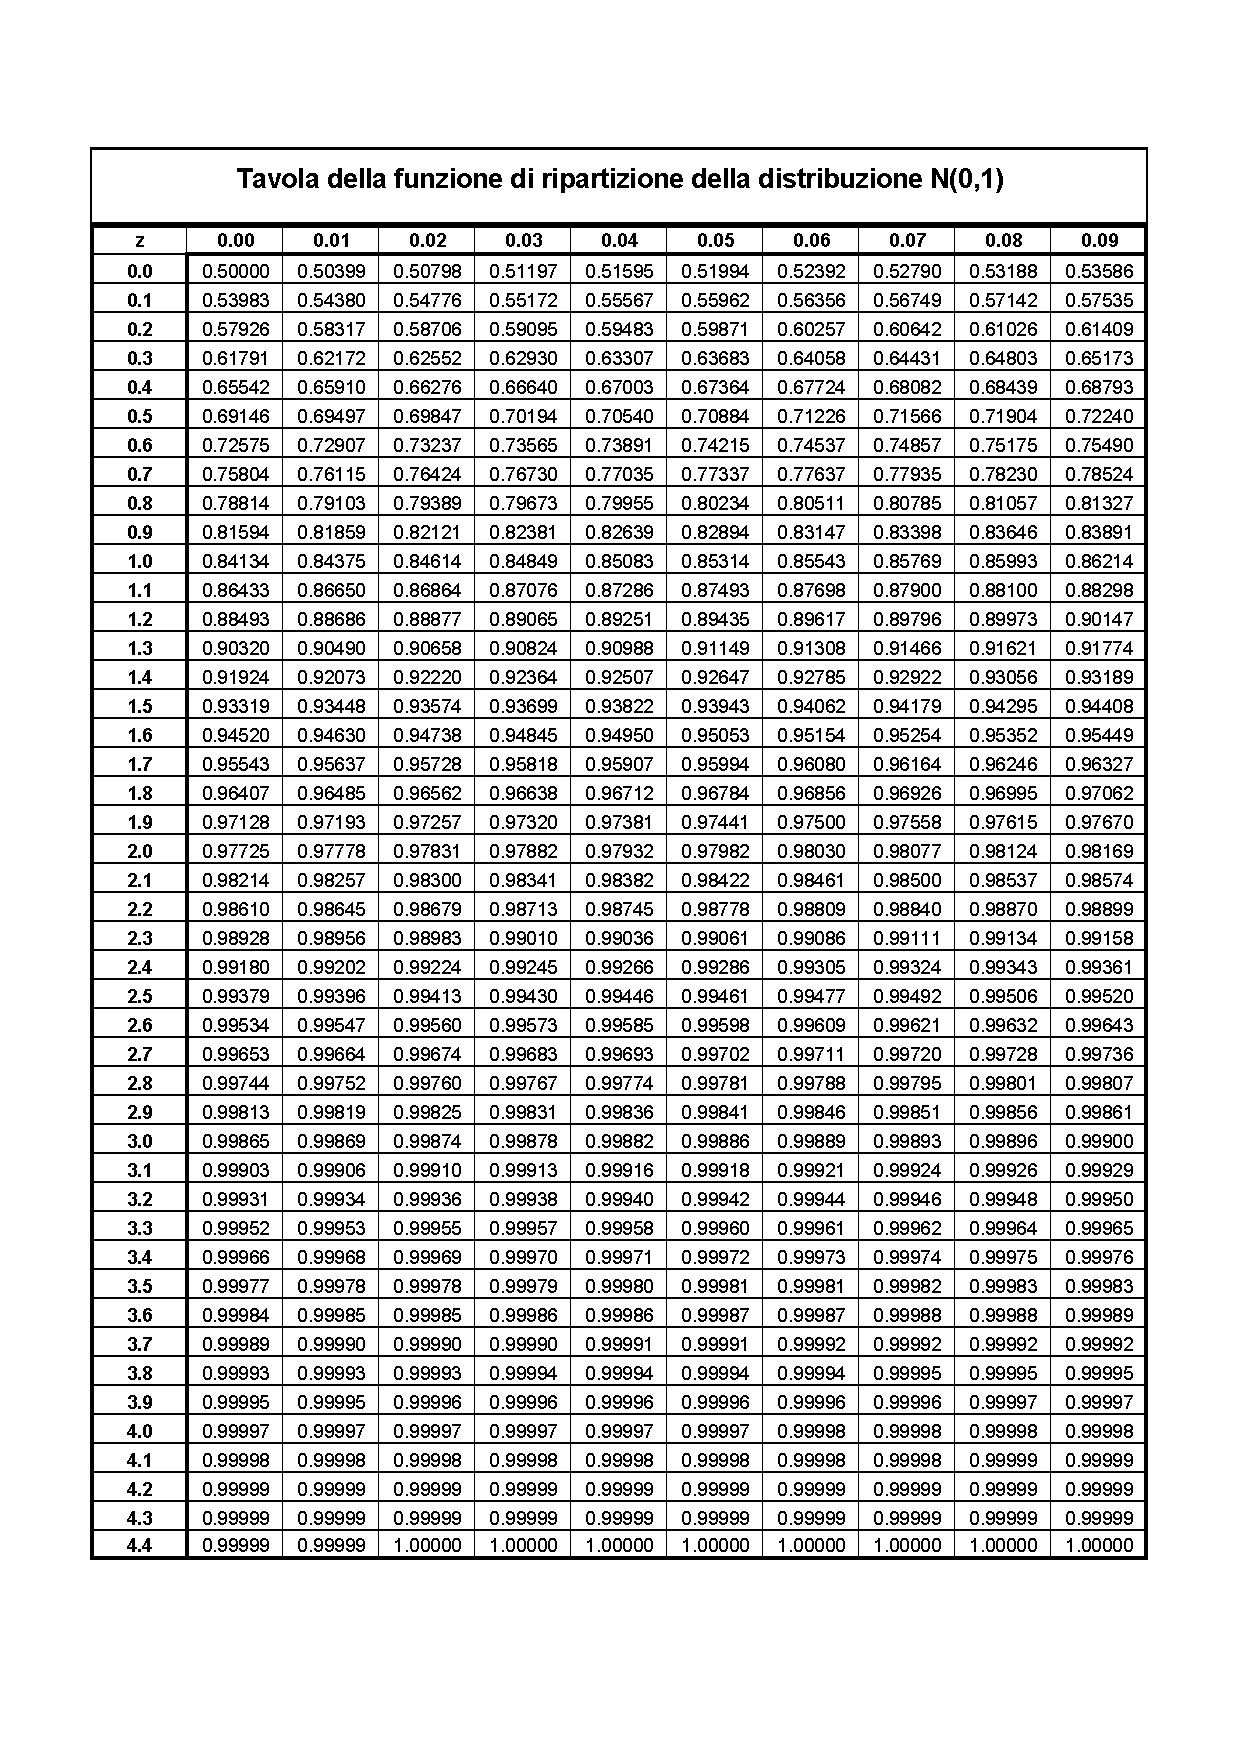
\includepdf[]{images/n01.pdf}

